%%%%%%%%%%%%%%%%%%%%%%%%%%%%%%%%%%%%%%%%%%%%%%
%%%%%%%%%%%%%%%%%%%%%%%%%%%%%%%%%%%%%%%%%%%%%%
%%			     Anexo B     			    %%
%%%%%%%%%%%%%%%%%%%%%%%%%%%%%%%%%%%%%%%%%%%%%%
%%%%%%%%%%%%%%%%%%%%%%%%%%%%%%%%%%%%%%%%%%%%%%
\chapter{Figuras} \label{anexoB}
\newpage

\section{Figuras}
\blindtext
\begin{figure}[htb]
	\centering
	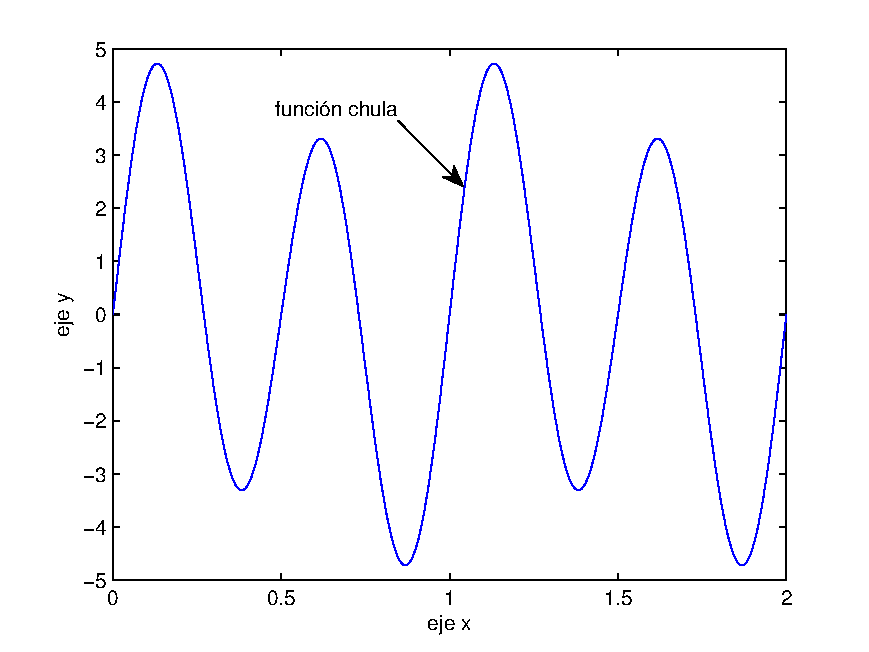
\includegraphics[width=0.7\linewidth]{anexo_b/figuras_dir/ejemplo-eps-converted-to.pdf}
	\caption{Figura en PDF}
	\label{FiguraB_1}
\end{figure} 

	\subsection{Figuras giradas}
	
	\blindtext	
	\blindtext
	\blindtext
	
	Para crear una Figura girada como la que se puede ver en la Fig. \ref{FiguraB_2} se usa la opción \verb|angle|.
	
	\begin{figure}[htb]
		\centering
		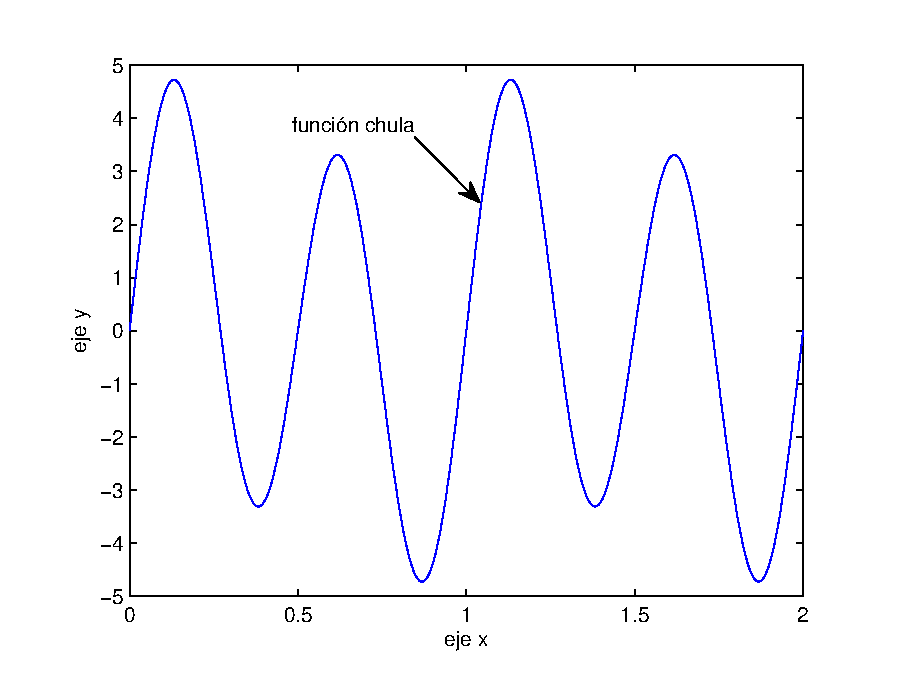
\includegraphics[width=0.7\linewidth,angle=90]{anexo_b/figuras_dir/ejemplo.eps}
		\caption{Figura en {\psverb+es\_currier+} y girada}
		\label{FiguraB_2}
	\end{figure} 

	La figura cuenta con el tipo de letra \verb|currier| en el pie de la figura, para ello se usar el comando {\psverb+psverb+}.
